\subsection{Matrici di similarità}
\label{ssec:mtrsim}
Si ipotizza che le frasi appartenenti allo stesso topic siano simili fra loro. Per verificare questa ipotesi è stato selezionato un campione random di 5 frasi per ogni topic, è stato effettuato l'embed delle frasi e poi fatto l'inner product degli embed.

Di seguito vengono mostrate le metrici di similarità ottenute dell'inner product. Si può notare che le matrici di similarità con i valori più alti sono:
\begin{itemize}
    \item politics(fig.\ref{fig:mtrsim_p}): con valori che vanno da 0.63 a 1
    \item job(fig.\ref{fig:mtrsim_j}): con valori che vanno da 0.72 a 1
I restanti invece presentano valori di similarità molto più bassi.

Infine è stata realizzata una matrice che metteva insieme tutti i vari topic per vedere quanto le frasi appartenenti a diversi topic si somigliassero. Il risultato è mostrato in fig.(\ref{fig:mtrsim_mix} dove si può notate che le celle colorate con toni chiari(valori superiori a 0.5) siano ottenute dalla intersezione di frasi appartenenti allo stesso topic, mentre, le celle colorate con topi scuri(valori inferiori al 0.5) siano data della intersezione di frasi appartenenti a topic diversi.
\end{itemize}
\begin{figure}[h!t]
    \centering
    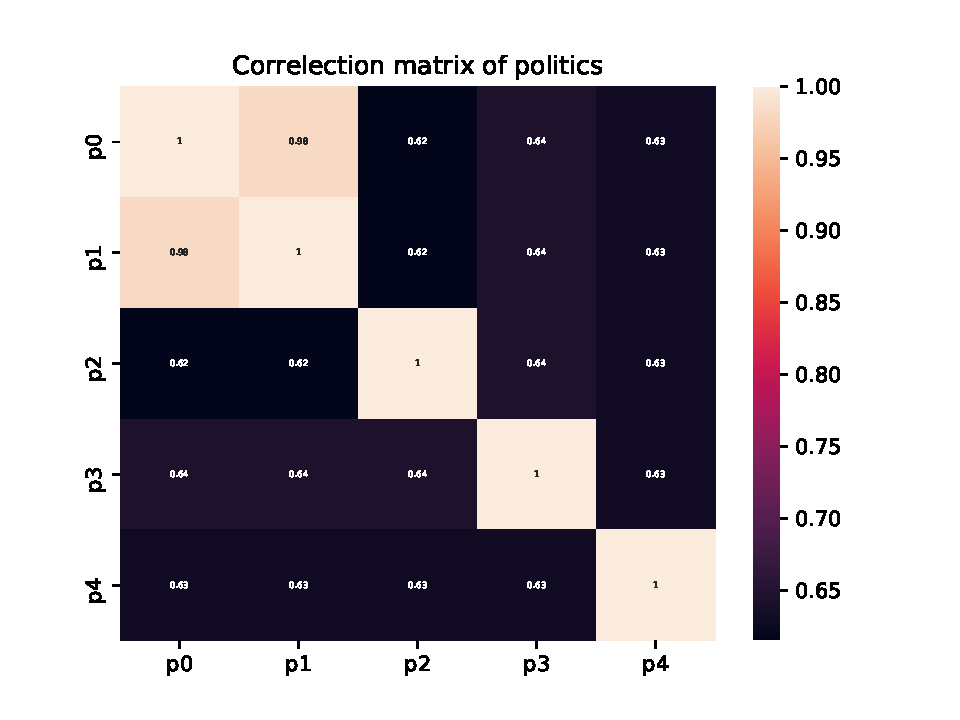
\includegraphics{Figure/simMatr/politics.pdf}
    \caption{matrici di similarità delle frasi appartenenti al topic politics}
    \label{fig:mtrsim_p}
\end{figure}
\FloatBarrier

\begin{figure}[h!t]
    \centering
    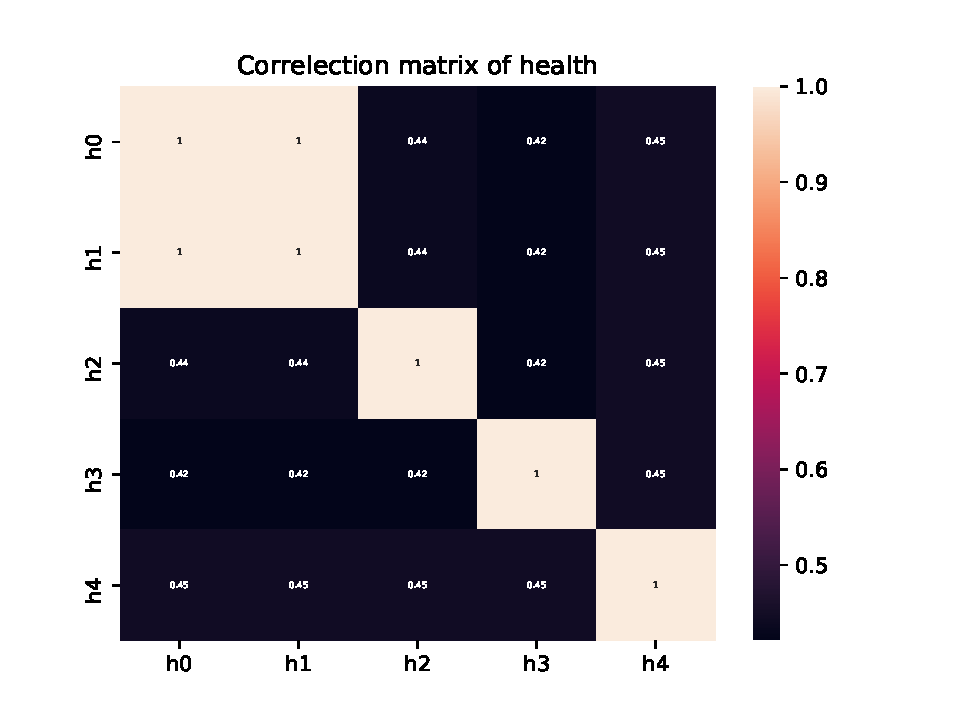
\includegraphics{Figure/simMatr/health.pdf}
    \caption{matrici di similarità delle frasi appartenenti al topic health}
    \label{fig:mtrsim_h}
\end{figure}
\FloatBarrier

\begin{figure}[h!t]
    \centering
    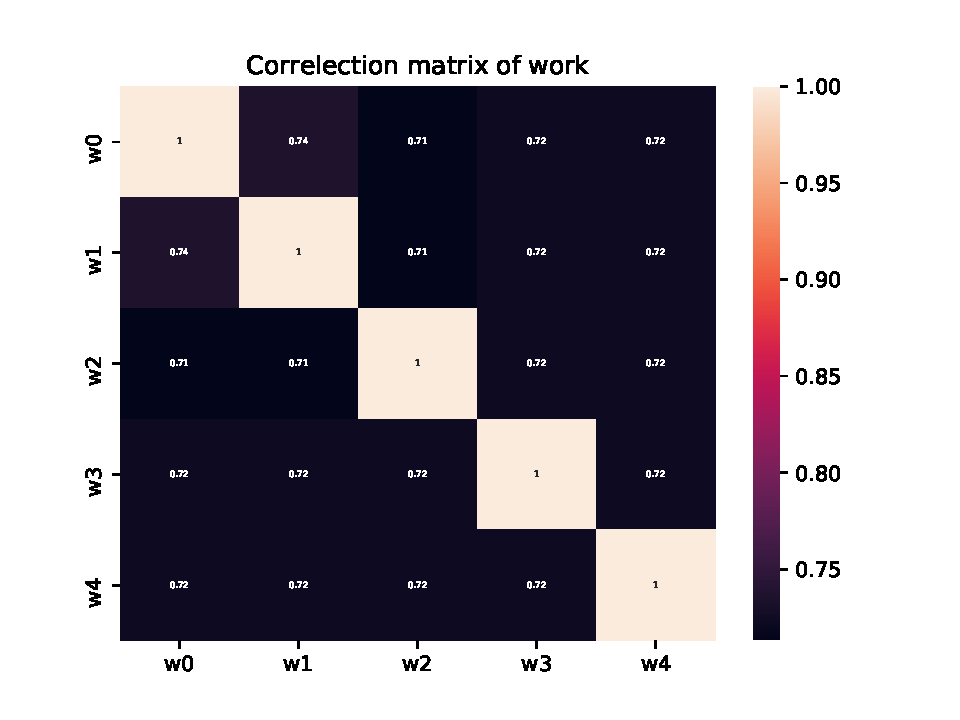
\includegraphics{Figure/simMatr/work.pdf}
    \caption{matrici di similarità delle frasi appartenenti al topic job}
    \label{fig:mtrsim_j}
\end{figure}
\FloatBarrier

\begin{figure}[h!t]
    \centering
    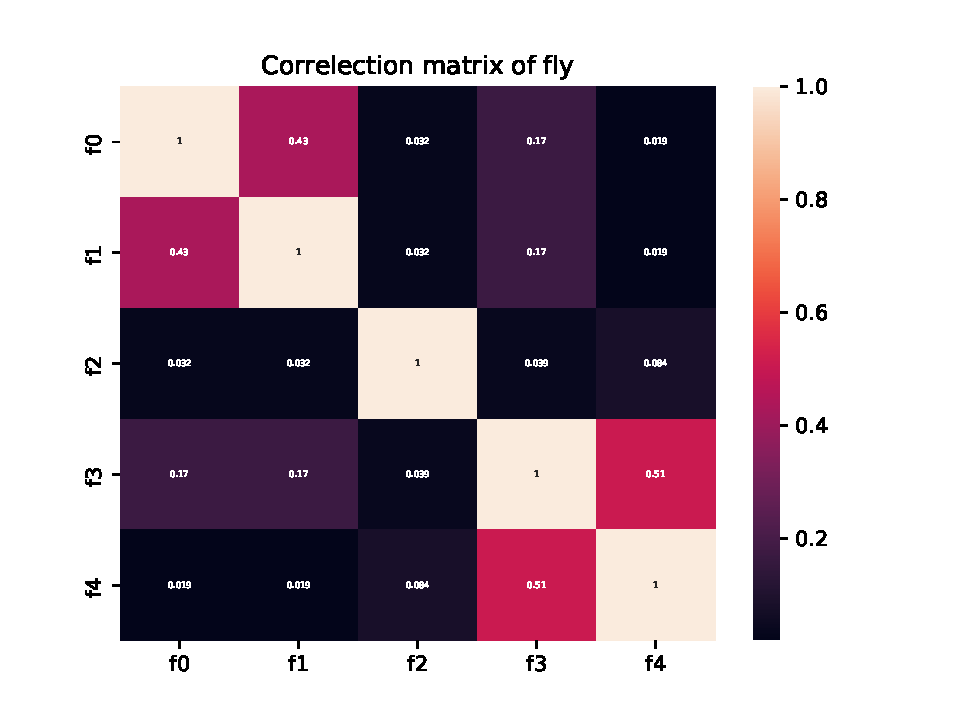
\includegraphics{Figure/simMatr/fly.pdf}
    \caption{matrici di similarità delle frasi appartenenti al topic travel}
    \label{fig:mtrsim_t}
\end{figure}
\FloatBarrier

\begin{figure}[h!t]
    \centering
    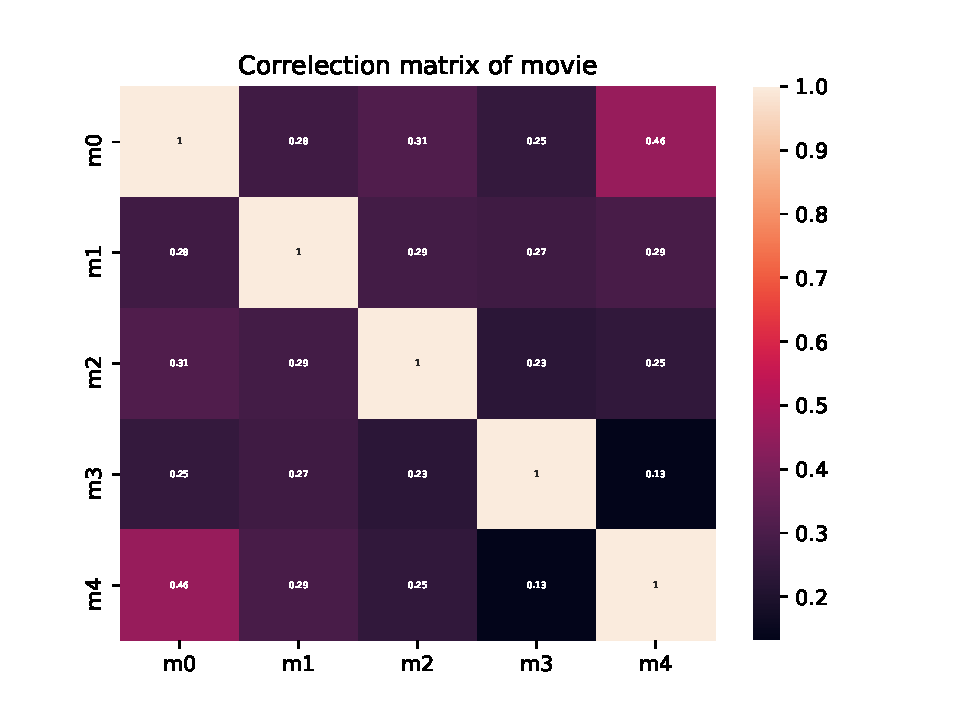
\includegraphics{Figure/simMatr/movie.pdf}
    \caption{matrici di similarità delle frasi appartenenti al topic general}
    \label{fig:mtrsim_g}
\end{figure}
\FloatBarrier

\begin{figure}[h!t]
    \centering
    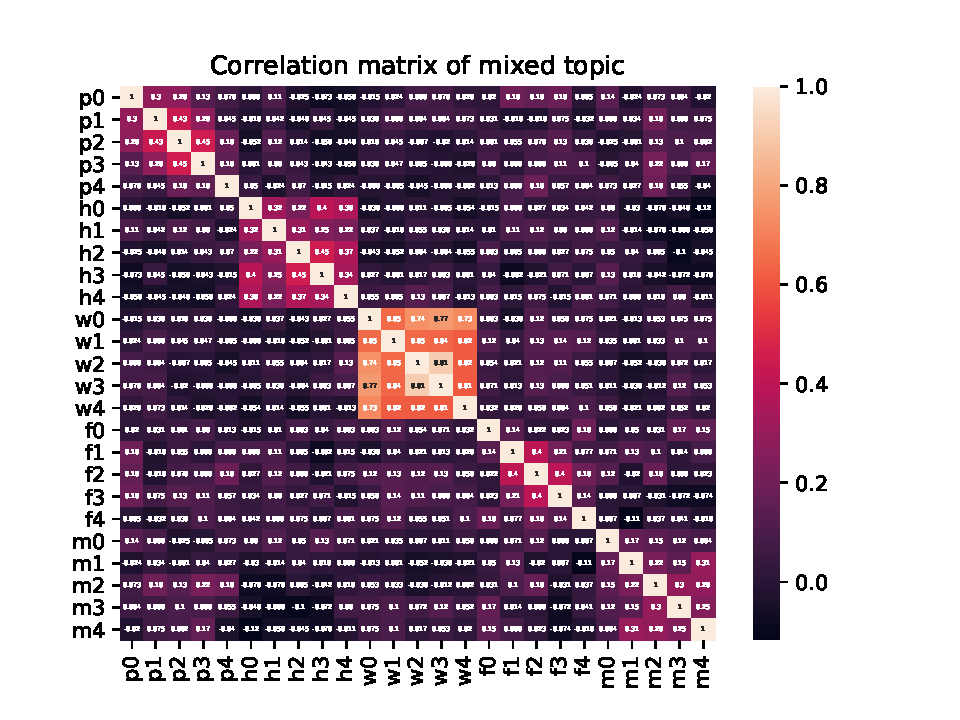
\includegraphics{Figure/simMatr/mixed.pdf}
    \caption{matrici di similarità delle frasi appartenenti ai diversi topic}
    \label{fig:mtrsim_mix}
\end{figure}
\FloatBarrier
